% !TeX program = lualatex -synctex=1 -interaction=nonstopmode --shell-escape %.tex
\documentclass[beamer,xcolor=dvipsnames]{standalone}
\RequirePackage[rus]{borochkin_tikz}

\newcolumntype{C}[1]{>{\centering\arraybackslash}p{#1}}
\newcolumntype{L}[1]{>{\raggedright\arraybackslash}p{#1}}

\begin{document}
\begin{standaloneframe}[shrink=0, fragile]
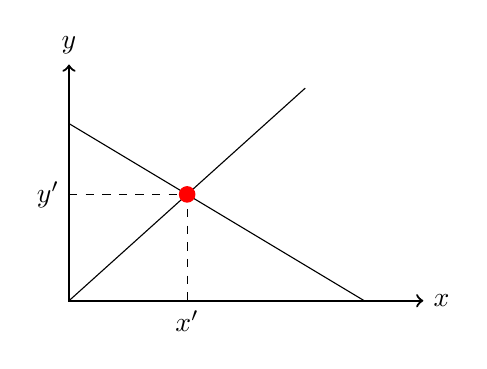
\begin{tikzpicture}[scale=1.5]
% Draw axes
\draw [<->,thick] (0,2) node (yaxis) [above] {$y$}
|- (3,0) node (xaxis) [right] {$x$};
% Draw two intersecting lines
\draw (0,0) coordinate (a_1) -- (2,1.8) coordinate (a_2);
\draw (0,1.5) coordinate (b_1) -- (2.5,0) coordinate (b_2);
% Calculate the intersection of the lines a_1 -- a_2 and b_1 -- b_2
% and store the coordinate in c.
\coordinate (c) at (intersection of a_1--a_2 and b_1--b_2);
% Draw lines indicating intersection with y and x axis. Here we use
% the perpendicular coordinate system
\draw[dashed] (yaxis |- c) node[left] {$y'$}
-| (xaxis -| c) node[below] {$x'$};
% Draw a dot to indicate intersection point
\fill[red] (c) circle (2pt);
\end{tikzpicture}
\end{standaloneframe}
\end{document}